\documentclass[twoside]{book}

% Packages required by doxygen
\usepackage{fixltx2e}
\usepackage{calc}
\usepackage{doxygen}
\usepackage[export]{adjustbox} % also loads graphicx
\usepackage{graphicx}
\usepackage[utf8]{inputenc}
\usepackage{makeidx}
\usepackage{multicol}
\usepackage{multirow}
\PassOptionsToPackage{warn}{textcomp}
\usepackage{textcomp}
\usepackage[nointegrals]{wasysym}
\usepackage[table]{xcolor}

% Font selection
\usepackage[T1]{fontenc}
\usepackage[scaled=.90]{helvet}
\usepackage{courier}
\usepackage{amssymb}
\usepackage{sectsty}
\renewcommand{\familydefault}{\sfdefault}
\allsectionsfont{%
  \fontseries{bc}\selectfont%
  \color{darkgray}%
}
\renewcommand{\DoxyLabelFont}{%
  \fontseries{bc}\selectfont%
  \color{darkgray}%
}
\newcommand{\+}{\discretionary{\mbox{\scriptsize$\hookleftarrow$}}{}{}}

% Page & text layout
\usepackage{geometry}
\geometry{%
  a4paper,%
  top=2.5cm,%
  bottom=2.5cm,%
  left=2.5cm,%
  right=2.5cm%
}
\tolerance=750
\hfuzz=15pt
\hbadness=750
\setlength{\emergencystretch}{15pt}
\setlength{\parindent}{0cm}
\setlength{\parskip}{3ex plus 2ex minus 2ex}
\makeatletter
\renewcommand{\paragraph}{%
  \@startsection{paragraph}{4}{0ex}{-1.0ex}{1.0ex}{%
    \normalfont\normalsize\bfseries\SS@parafont%
  }%
}
\renewcommand{\subparagraph}{%
  \@startsection{subparagraph}{5}{0ex}{-1.0ex}{1.0ex}{%
    \normalfont\normalsize\bfseries\SS@subparafont%
  }%
}
\makeatother

% Headers & footers
\usepackage{fancyhdr}
\pagestyle{fancyplain}
\fancyhead[LE]{\fancyplain{}{\bfseries\thepage}}
\fancyhead[CE]{\fancyplain{}{}}
\fancyhead[RE]{\fancyplain{}{\bfseries\leftmark}}
\fancyhead[LO]{\fancyplain{}{\bfseries\rightmark}}
\fancyhead[CO]{\fancyplain{}{}}
\fancyhead[RO]{\fancyplain{}{\bfseries\thepage}}
\fancyfoot[LE]{\fancyplain{}{}}
\fancyfoot[CE]{\fancyplain{}{}}
\fancyfoot[RE]{\fancyplain{}{\bfseries\scriptsize Generated by Doxygen }}
\fancyfoot[LO]{\fancyplain{}{\bfseries\scriptsize Generated by Doxygen }}
\fancyfoot[CO]{\fancyplain{}{}}
\fancyfoot[RO]{\fancyplain{}{}}
\renewcommand{\footrulewidth}{0.4pt}
\renewcommand{\chaptermark}[1]{%
  \markboth{#1}{}%
}
\renewcommand{\sectionmark}[1]{%
  \markright{\thesection\ #1}%
}

% Indices & bibliography
\usepackage{natbib}
\usepackage[titles]{tocloft}
\setcounter{tocdepth}{3}
\setcounter{secnumdepth}{5}
\makeindex

% Hyperlinks (required, but should be loaded last)
\usepackage{ifpdf}
\ifpdf
  \usepackage[pdftex,pagebackref=true]{hyperref}
\else
  \usepackage[ps2pdf,pagebackref=true]{hyperref}
\fi
\hypersetup{%
  colorlinks=true,%
  linkcolor=blue,%
  citecolor=blue,%
  unicode%
}

% Custom commands
\newcommand{\clearemptydoublepage}{%
  \newpage{\pagestyle{empty}\cleardoublepage}%
}

\usepackage{caption}
\captionsetup{labelsep=space,justification=centering,font={bf},singlelinecheck=off,skip=4pt,position=top}

%===== C O N T E N T S =====

\begin{document}

% Titlepage & ToC
\hypersetup{pageanchor=false,
             bookmarksnumbered=true,
             pdfencoding=unicode
            }
\pagenumbering{alph}
\begin{titlepage}
\vspace*{7cm}
\begin{center}%
{\Large My Project }\\
\vspace*{1cm}
{\large Generated by Doxygen 1.8.13}\\
\end{center}
\end{titlepage}
\clearemptydoublepage
\pagenumbering{roman}
\tableofcontents
\clearemptydoublepage
\pagenumbering{arabic}
\hypersetup{pageanchor=true}

%--- Begin generated contents ---
\chapter{CS 202 Semester Project Template}
\label{index}\hypertarget{index}{}\input{index}
\chapter{Hierarchical Index}
\section{Class Hierarchy}
This inheritance list is sorted roughly, but not completely, alphabetically\+:\begin{DoxyCompactList}
\item \contentsline{section}{Driver}{\pageref{classDriver}}{}
\item \contentsline{section}{I\+Algorithm$<$ T $>$}{\pageref{classIAlgorithm}}{}
\begin{DoxyCompactList}
\item \contentsline{section}{Echo$<$ T $>$}{\pageref{classEcho}}{}
\item \contentsline{section}{Noisegate$<$ T $>$}{\pageref{classNoisegate}}{}
\item \contentsline{section}{Normalization$<$ T $>$}{\pageref{classNormalization}}{}
\end{DoxyCompactList}
\item \contentsline{section}{Metadata}{\pageref{classMetadata}}{}
\item \contentsline{section}{Metadata\+Header}{\pageref{structMetadataHeader}}{}
\item \contentsline{section}{Metadata\+Manager}{\pageref{classMetadataManager}}{}
\item \contentsline{section}{Wav}{\pageref{classWav}}{}
\item \contentsline{section}{Wav\+Header}{\pageref{structWavHeader}}{}
\item \contentsline{section}{Wav\+Manager}{\pageref{classWavManager}}{}
\end{DoxyCompactList}

\chapter{Class Index}
\section{Class List}
Here are the classes, structs, unions and interfaces with brief descriptions\+:\begin{DoxyCompactList}
\item\contentsline{section}{\hyperlink{classDriver}{Driver} }{\pageref{classDriver}}{}
\item\contentsline{section}{\hyperlink{classEcho}{Echo$<$ T $>$} }{\pageref{classEcho}}{}
\item\contentsline{section}{\hyperlink{classIAlgorithm}{I\+Algorithm$<$ T $>$} }{\pageref{classIAlgorithm}}{}
\item\contentsline{section}{\hyperlink{classMetadata}{Metadata} }{\pageref{classMetadata}}{}
\item\contentsline{section}{\hyperlink{structMetadataHeader}{Metadata\+Header} }{\pageref{structMetadataHeader}}{}
\item\contentsline{section}{\hyperlink{classMetadataManager}{Metadata\+Manager} }{\pageref{classMetadataManager}}{}
\item\contentsline{section}{\hyperlink{classNoisegate}{Noisegate$<$ T $>$} }{\pageref{classNoisegate}}{}
\item\contentsline{section}{\hyperlink{classNormalization}{Normalization$<$ T $>$} }{\pageref{classNormalization}}{}
\item\contentsline{section}{\hyperlink{classWav}{Wav} }{\pageref{classWav}}{}
\item\contentsline{section}{\hyperlink{structWavHeader}{Wav\+Header} }{\pageref{structWavHeader}}{}
\item\contentsline{section}{\hyperlink{classWavManager}{Wav\+Manager} }{\pageref{classWavManager}}{}
\end{DoxyCompactList}

\chapter{File Index}
\section{File List}
Here is a list of all documented files with brief descriptions\+:\begin{DoxyCompactList}
\item\contentsline{section}{{\bfseries Driver.\+h} }{\pageref{Driver_8h}}{}
\item\contentsline{section}{{\bfseries Echo.\+h} }{\pageref{Echo_8h}}{}
\item\contentsline{section}{{\bfseries I\+Algorithm.\+h} }{\pageref{IAlgorithm_8h}}{}
\item\contentsline{section}{\hyperlink{main_8cpp}{main.\+cpp} }{\pageref{main_8cpp}}{}
\item\contentsline{section}{{\bfseries Metadata.\+h} }{\pageref{Metadata_8h}}{}
\item\contentsline{section}{{\bfseries Metadata\+Header.\+h} }{\pageref{MetadataHeader_8h}}{}
\item\contentsline{section}{{\bfseries Metadata\+Manager.\+h} }{\pageref{MetadataManager_8h}}{}
\item\contentsline{section}{{\bfseries Noisegate.\+h} }{\pageref{Noisegate_8h}}{}
\item\contentsline{section}{{\bfseries Normalization.\+h} }{\pageref{Normalization_8h}}{}
\item\contentsline{section}{{\bfseries Wav.\+h} }{\pageref{Wav_8h}}{}
\item\contentsline{section}{{\bfseries Wav\+Header.\+h} }{\pageref{WavHeader_8h}}{}
\item\contentsline{section}{{\bfseries Wav\+Manager.\+h} }{\pageref{WavManager_8h}}{}
\end{DoxyCompactList}

\chapter{Class Documentation}
\hypertarget{classDriver}{}\section{Driver Class Reference}
\label{classDriver}\index{Driver@{Driver}}
\subsection*{Public Member Functions}
\begin{DoxyCompactItemize}
\item 
\mbox{\Hypertarget{classDriver_add5a6c755a1e845cc3d7c0cd7e7fbc17}\label{classDriver_add5a6c755a1e845cc3d7c0cd7e7fbc17}} 
{\bfseries Driver} (\hyperlink{classWav}{Wav} $\ast$wav)
\item 
void \hyperlink{classDriver_a5d58141395b60701ae65d3623c3053f6}{set\+Wav} (\hyperlink{classWav}{Wav} $\ast$)
\item 
void \hyperlink{classDriver_a7b8110d43dc29e26fec11f4120693714}{process\+Wav} ()
\item 
void \hyperlink{classDriver_a43544d196cd4055dced0c0ef654ffd62}{output\+Wav\+File} (std\+::vector$<$ std\+::string $>$)
\item 
void \hyperlink{classDriver_ab6ac2a7b99e934cf8a3c5ebe229eb63b}{output\+C\+S\+V\+File} (std\+::vector$<$ \hyperlink{classWav}{Wav} $\ast$$>$)
\item 
void \hyperlink{classDriver_a23d1437a01106d70634aed9271b44e49}{edit\+Metadata} ()
\end{DoxyCompactItemize}


\subsection{Member Function Documentation}
\mbox{\Hypertarget{classDriver_a23d1437a01106d70634aed9271b44e49}\label{classDriver_a23d1437a01106d70634aed9271b44e49}} 
\index{Driver@{Driver}!edit\+Metadata@{edit\+Metadata}}
\index{edit\+Metadata@{edit\+Metadata}!Driver@{Driver}}
\subsubsection{\texorpdfstring{edit\+Metadata()}{editMetadata()}}
{\footnotesize\ttfamily void Driver\+::edit\+Metadata (\begin{DoxyParamCaption}{ }\end{DoxyParamCaption})}

edit metadata \mbox{\Hypertarget{classDriver_ab6ac2a7b99e934cf8a3c5ebe229eb63b}\label{classDriver_ab6ac2a7b99e934cf8a3c5ebe229eb63b}} 
\index{Driver@{Driver}!output\+C\+S\+V\+File@{output\+C\+S\+V\+File}}
\index{output\+C\+S\+V\+File@{output\+C\+S\+V\+File}!Driver@{Driver}}
\subsubsection{\texorpdfstring{output\+C\+S\+V\+File()}{outputCSVFile()}}
{\footnotesize\ttfamily void Driver\+::output\+C\+S\+V\+File (\begin{DoxyParamCaption}\item[{std\+::vector$<$ \hyperlink{classWav}{Wav} $\ast$$>$}]{wavs }\end{DoxyParamCaption})}

writes \hyperlink{classWav}{Wav} file to output .csv file 
\begin{DoxyParams}{Parameters}
{\em wavs} & vector of pointer to \hyperlink{classWav}{Wav} files in directory \\
\hline
\end{DoxyParams}
\mbox{\Hypertarget{classDriver_a43544d196cd4055dced0c0ef654ffd62}\label{classDriver_a43544d196cd4055dced0c0ef654ffd62}} 
\index{Driver@{Driver}!output\+Wav\+File@{output\+Wav\+File}}
\index{output\+Wav\+File@{output\+Wav\+File}!Driver@{Driver}}
\subsubsection{\texorpdfstring{output\+Wav\+File()}{outputWavFile()}}
{\footnotesize\ttfamily void Driver\+::output\+Wav\+File (\begin{DoxyParamCaption}\item[{std\+::vector$<$ std\+::string $>$}]{file\+Names }\end{DoxyParamCaption})}

writes \hyperlink{classWav}{Wav} file to output .wav file 
\begin{DoxyParams}{Parameters}
{\em files} & vector of filenames in directory \\
\hline
\end{DoxyParams}
\mbox{\Hypertarget{classDriver_a7b8110d43dc29e26fec11f4120693714}\label{classDriver_a7b8110d43dc29e26fec11f4120693714}} 
\index{Driver@{Driver}!process\+Wav@{process\+Wav}}
\index{process\+Wav@{process\+Wav}!Driver@{Driver}}
\subsubsection{\texorpdfstring{process\+Wav()}{processWav()}}
{\footnotesize\ttfamily void Driver\+::process\+Wav (\begin{DoxyParamCaption}{ }\end{DoxyParamCaption})}

handles \hyperlink{classWav}{Wav} processing sequence \mbox{\Hypertarget{classDriver_a5d58141395b60701ae65d3623c3053f6}\label{classDriver_a5d58141395b60701ae65d3623c3053f6}} 
\index{Driver@{Driver}!set\+Wav@{set\+Wav}}
\index{set\+Wav@{set\+Wav}!Driver@{Driver}}
\subsubsection{\texorpdfstring{set\+Wav()}{setWav()}}
{\footnotesize\ttfamily void Driver\+::set\+Wav (\begin{DoxyParamCaption}\item[{\hyperlink{classWav}{Wav} $\ast$}]{wav }\end{DoxyParamCaption})}


\begin{DoxyItemize}
\item sets \hyperlink{classWav}{Wav} pointer in \hyperlink{classDriver}{Driver} 
\end{DoxyItemize}

The documentation for this class was generated from the following files\+:\begin{DoxyCompactItemize}
\item 
Driver.\+h\item 
Driver.\+cpp\end{DoxyCompactItemize}

\hypertarget{classEcho}{}\section{Echo$<$ T $>$ Class Template Reference}
\label{classEcho}\index{Echo$<$ T $>$@{Echo$<$ T $>$}}


{\ttfamily \#include $<$Echo.\+h$>$}



Inheritance diagram for Echo$<$ T $>$\+:
\nopagebreak
\begin{figure}[H]
\begin{center}
\leavevmode
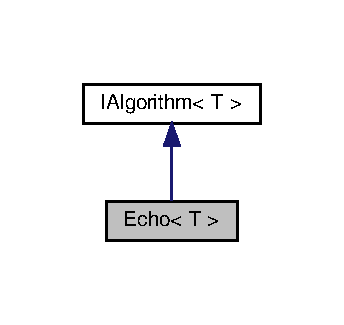
\includegraphics[width=165pt]{d1/dd3/classEcho__inherit__graph}
\end{center}
\end{figure}


Collaboration diagram for Echo$<$ T $>$\+:
\nopagebreak
\begin{figure}[H]
\begin{center}
\leavevmode
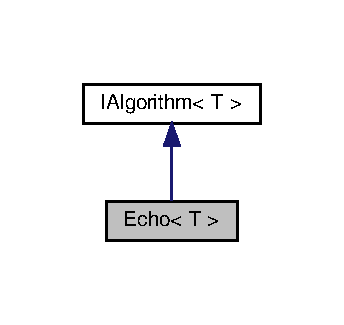
\includegraphics[width=165pt]{da/d44/classEcho__coll__graph}
\end{center}
\end{figure}
\subsection*{Public Member Functions}
\begin{DoxyCompactItemize}
\item 
\hyperlink{classEcho_af348cd7f23248e72046c5d006d3adca7}{Echo} (int delay)
\item 
void \hyperlink{classEcho_af5ea3baaa51600cf111f21f931895b46}{process\+Buffer} (T $\ast$buffer, int buffer\+Size) override
\end{DoxyCompactItemize}


\subsection{Detailed Description}
\subsubsection*{template$<$typename T$>$\newline
class Echo$<$ T $>$}

Authors\+: Parker True, Chris Fernandez, \& Ilana Macy Date Due\+: May 2, 2021 Assignment\+: Semester Project

applies echo effect to \hyperlink{classWav}{Wav} based on input delay 

\subsection{Constructor \& Destructor Documentation}
\mbox{\Hypertarget{classEcho_af348cd7f23248e72046c5d006d3adca7}\label{classEcho_af348cd7f23248e72046c5d006d3adca7}} 
\index{Echo@{Echo}!Echo@{Echo}}
\index{Echo@{Echo}!Echo@{Echo}}
\subsubsection{\texorpdfstring{Echo()}{Echo()}}
{\footnotesize\ttfamily template$<$typename T $>$ \\
\hyperlink{classEcho}{Echo}$<$ T $>$\+::\hyperlink{classEcho}{Echo} (\begin{DoxyParamCaption}\item[{int}]{delay }\end{DoxyParamCaption})\hspace{0.3cm}{\ttfamily [inline]}, {\ttfamily [explicit]}}

constructs \hyperlink{classEcho}{Echo} processor 
\begin{DoxyParams}{Parameters}
{\em delay} & delay specified by user input \\
\hline
\end{DoxyParams}


\subsection{Member Function Documentation}
\mbox{\Hypertarget{classEcho_af5ea3baaa51600cf111f21f931895b46}\label{classEcho_af5ea3baaa51600cf111f21f931895b46}} 
\index{Echo@{Echo}!process\+Buffer@{process\+Buffer}}
\index{process\+Buffer@{process\+Buffer}!Echo@{Echo}}
\subsubsection{\texorpdfstring{process\+Buffer()}{processBuffer()}}
{\footnotesize\ttfamily template$<$typename T $>$ \\
void \hyperlink{classEcho}{Echo}$<$ T $>$\+::process\+Buffer (\begin{DoxyParamCaption}\item[{T $\ast$}]{buffer,  }\item[{int}]{buffer\+Size }\end{DoxyParamCaption})\hspace{0.3cm}{\ttfamily [inline]}, {\ttfamily [override]}, {\ttfamily [virtual]}}


\begin{DoxyParams}{Parameters}
{\em buffer} & pointer to audio buffer of type T \\
\hline
{\em buffer\+Size} & number of elements in audio buffer\\
\hline
\end{DoxyParams}
applies echo algorithm 

Implements \hyperlink{classIAlgorithm}{I\+Algorithm$<$ T $>$}.



The documentation for this class was generated from the following file\+:\begin{DoxyCompactItemize}
\item 
Echo.\+h\end{DoxyCompactItemize}

\hypertarget{classIAlgorithm}{}\section{I\+Algorithm$<$ T $>$ Class Template Reference}
\label{classIAlgorithm}\index{I\+Algorithm$<$ T $>$@{I\+Algorithm$<$ T $>$}}


{\ttfamily \#include $<$I\+Algorithm.\+h$>$}



Inheritance diagram for I\+Algorithm$<$ T $>$\+:
% FIG 0
\subsection*{Public Member Functions}
\begin{DoxyCompactItemize}
\item 
\mbox{\Hypertarget{classIAlgorithm_af5d33413d39ce61d543a73f951a4a4eb}\label{classIAlgorithm_af5d33413d39ce61d543a73f951a4a4eb}} 
virtual void {\bfseries process\+Buffer} (T $\ast$buffer, int buffer\+Size)=0
\end{DoxyCompactItemize}


\subsection{Detailed Description}
\subsubsection*{template$<$typename T$>$\newline
class I\+Algorithm$<$ T $>$}


\begin{DoxyItemize}
\item base template for processor algorithms \begin{DoxyNote}{Note}
-\/ Z\+E\+RO is located at 128 for unsigned chars, 0 for everything else 

L\+O\+W\+ER and U\+P\+P\+ER are in relation to adjusted value (after substracting Z\+E\+RO) for unsigned chars 
\end{DoxyNote}

\end{DoxyItemize}

The documentation for this class was generated from the following file\+:\begin{DoxyCompactItemize}
\item 
I\+Algorithm.\+h\end{DoxyCompactItemize}

\hypertarget{classMetadata}{}\section{Metadata Class Reference}
\label{classMetadata}\index{Metadata@{Metadata}}


{\ttfamily \#include $<$Metadata.\+h$>$}

\subsection*{Public Member Functions}
\begin{DoxyCompactItemize}
\item 
\hyperlink{classMetadata_a1877568b5463425c93532224b6bf6950}{Metadata} (std\+::ifstream \&)
\item 
std\+::string \hyperlink{classMetadata_a3567498d73b473be0b3d6ba505067f9c}{get\+ID} () const
\item 
int \hyperlink{classMetadata_a358f06aba81e46be0f8deb7bb69b1f01}{get\+Size} () const
\item 
int \hyperlink{classMetadata_a039be0a66dabf1ea223790066ab6d430}{calc\+Size} ()
\item 
std\+::string \hyperlink{classMetadata_a59e34c51d464ab8e123e28abf8ef2e67}{get\+Buffer} () const
\item 
void \hyperlink{classMetadata_ae117e7b7973744baeb0faac3db705ba0}{set\+Buffer} (std\+::string)
\item 
void \hyperlink{classMetadata_a940cbd072f1b20e8f4c81806bad87f2c}{write\+File} (std\+::ofstream \&)
\end{DoxyCompactItemize}


\subsection{Detailed Description}
Authors\+: Parker True, Chris Fernandez, \& Ilana Macy Date Due\+: May 2, 2021 Assignment\+: Semester Project 

\subsection{Constructor \& Destructor Documentation}
\mbox{\Hypertarget{classMetadata_a1877568b5463425c93532224b6bf6950}\label{classMetadata_a1877568b5463425c93532224b6bf6950}} 
\index{Metadata@{Metadata}!Metadata@{Metadata}}
\index{Metadata@{Metadata}!Metadata@{Metadata}}
\subsubsection{\texorpdfstring{Metadata()}{Metadata()}}
{\footnotesize\ttfamily Metadata\+::\+Metadata (\begin{DoxyParamCaption}\item[{std\+::ifstream \&}]{file }\end{DoxyParamCaption})}

constructs one metadata chunk from input file 

\subsection{Member Function Documentation}
\mbox{\Hypertarget{classMetadata_a039be0a66dabf1ea223790066ab6d430}\label{classMetadata_a039be0a66dabf1ea223790066ab6d430}} 
\index{Metadata@{Metadata}!calc\+Size@{calc\+Size}}
\index{calc\+Size@{calc\+Size}!Metadata@{Metadata}}
\subsubsection{\texorpdfstring{calc\+Size()}{calcSize()}}
{\footnotesize\ttfamily int Metadata\+::calc\+Size (\begin{DoxyParamCaption}{ }\end{DoxyParamCaption})}

\begin{DoxyReturn}{Returns}
-\/ number of bytes in metadata buffer 
\end{DoxyReturn}
\mbox{\Hypertarget{classMetadata_a59e34c51d464ab8e123e28abf8ef2e67}\label{classMetadata_a59e34c51d464ab8e123e28abf8ef2e67}} 
\index{Metadata@{Metadata}!get\+Buffer@{get\+Buffer}}
\index{get\+Buffer@{get\+Buffer}!Metadata@{Metadata}}
\subsubsection{\texorpdfstring{get\+Buffer()}{getBuffer()}}
{\footnotesize\ttfamily std\+::string Metadata\+::get\+Buffer (\begin{DoxyParamCaption}{ }\end{DoxyParamCaption}) const}

\begin{DoxyReturn}{Returns}
-\/ metadata buffer 
\end{DoxyReturn}
\mbox{\Hypertarget{classMetadata_a3567498d73b473be0b3d6ba505067f9c}\label{classMetadata_a3567498d73b473be0b3d6ba505067f9c}} 
\index{Metadata@{Metadata}!get\+ID@{get\+ID}}
\index{get\+ID@{get\+ID}!Metadata@{Metadata}}
\subsubsection{\texorpdfstring{get\+I\+D()}{getID()}}
{\footnotesize\ttfamily std\+::string Metadata\+::get\+ID (\begin{DoxyParamCaption}{ }\end{DoxyParamCaption}) const}

\begin{DoxyReturn}{Returns}
-\/ metadata ID as string 
\end{DoxyReturn}
\mbox{\Hypertarget{classMetadata_a358f06aba81e46be0f8deb7bb69b1f01}\label{classMetadata_a358f06aba81e46be0f8deb7bb69b1f01}} 
\index{Metadata@{Metadata}!get\+Size@{get\+Size}}
\index{get\+Size@{get\+Size}!Metadata@{Metadata}}
\subsubsection{\texorpdfstring{get\+Size()}{getSize()}}
{\footnotesize\ttfamily int Metadata\+::get\+Size (\begin{DoxyParamCaption}{ }\end{DoxyParamCaption}) const}

\begin{DoxyReturn}{Returns}
-\/ number of bytes in metadata size variable 
\end{DoxyReturn}
\mbox{\Hypertarget{classMetadata_ae117e7b7973744baeb0faac3db705ba0}\label{classMetadata_ae117e7b7973744baeb0faac3db705ba0}} 
\index{Metadata@{Metadata}!set\+Buffer@{set\+Buffer}}
\index{set\+Buffer@{set\+Buffer}!Metadata@{Metadata}}
\subsubsection{\texorpdfstring{set\+Buffer()}{setBuffer()}}
{\footnotesize\ttfamily void Metadata\+::set\+Buffer (\begin{DoxyParamCaption}\item[{std\+::string}]{buffer }\end{DoxyParamCaption})}


\begin{DoxyItemize}
\item sets metadata buffer when given a string 
\begin{DoxyParams}{Parameters}
{\em buffer} & -\/ the buffer \\
\hline
\end{DoxyParams}
\begin{DoxyNote}{Note}
-\/ when setting buffer we must update list\+Size in \hyperlink{structMetadataHeader}{Metadata\+Header} and file\+Size in \hyperlink{structWavHeader}{Wav\+Header} 
\end{DoxyNote}

\end{DoxyItemize}\mbox{\Hypertarget{classMetadata_a940cbd072f1b20e8f4c81806bad87f2c}\label{classMetadata_a940cbd072f1b20e8f4c81806bad87f2c}} 
\index{Metadata@{Metadata}!write\+File@{write\+File}}
\index{write\+File@{write\+File}!Metadata@{Metadata}}
\subsubsection{\texorpdfstring{write\+File()}{writeFile()}}
{\footnotesize\ttfamily void Metadata\+::write\+File (\begin{DoxyParamCaption}\item[{std\+::ofstream \&}]{out\+File }\end{DoxyParamCaption})}


\begin{DoxyParams}{Parameters}
{\em out\+File} & output file stream\\
\hline
\end{DoxyParams}
writes one busy piece 

The documentation for this class was generated from the following files\+:\begin{DoxyCompactItemize}
\item 
Metadata.\+h\item 
Metadata.\+cpp\end{DoxyCompactItemize}

\hypertarget{structMetadataHeader}{}\section{Metadata\+Header Struct Reference}
\label{structMetadataHeader}\index{Metadata\+Header@{Metadata\+Header}}


{\ttfamily \#include $<$Metadata\+Header.\+h$>$}



Collaboration diagram for Metadata\+Header\+:
% FIG 0
\subsection*{Public Attributes}
\begin{DoxyCompactItemize}
\item 
\mbox{\Hypertarget{structMetadataHeader_ac337fc72c9ae30daa7e2e9df57cbf08c}\label{structMetadataHeader_ac337fc72c9ae30daa7e2e9df57cbf08c}} 
char {\bfseries list\+ID} \mbox{[}4\mbox{]}
\item 
\mbox{\Hypertarget{structMetadataHeader_ad3bf1dfe7faecd43c79d3d9c81319e2b}\label{structMetadataHeader_ad3bf1dfe7faecd43c79d3d9c81319e2b}} 
int {\bfseries list\+Size}
\item 
\mbox{\Hypertarget{structMetadataHeader_aee40eba0102ce906a77af6ce2f344b44}\label{structMetadataHeader_aee40eba0102ce906a77af6ce2f344b44}} 
char {\bfseries info\+ID} \mbox{[}4\mbox{]}
\item 
\mbox{\Hypertarget{structMetadataHeader_a4e9ac5e747d9d24bea5f0675fd243540}\label{structMetadataHeader_a4e9ac5e747d9d24bea5f0675fd243540}} 
\hyperlink{classMetadataManager}{Metadata\+Manager} {\bfseries mm}
\end{DoxyCompactItemize}


\subsection{Detailed Description}
Authors\+: Parker True, Chris Fernandez, \& Ilana Macy Date Due\+: May 2, 2021 Assignment\+: Semester Project 

The documentation for this struct was generated from the following file\+:\begin{DoxyCompactItemize}
\item 
Metadata\+Header.\+h\end{DoxyCompactItemize}

\hypertarget{classMetadataManager}{}\section{Metadata\+Manager Class Reference}
\label{classMetadataManager}\index{Metadata\+Manager@{Metadata\+Manager}}


{\ttfamily \#include $<$Metadata\+Manager.\+h$>$}

\subsection*{Public Member Functions}
\begin{DoxyCompactItemize}
\item 
\hyperlink{classMetadataManager_ae78ad769dbe26e0e2cbab6548f7b6830}{Metadata\+Manager} (std\+::ifstream \&)
\item 
void \hyperlink{classMetadataManager_a4eb5b8e9539b2e158cacdd1bca2cacd9}{print} ()
\item 
int \hyperlink{classMetadataManager_a497d7031313fd7c43b11228145e927c2}{get\+Size} () const
\item 
void \hyperlink{classMetadataManager_ab67fbd206d6baa6e8c7e623564ca5f29}{write\+File} (std\+::ofstream \&)
\item 
void \hyperlink{classMetadataManager_a0a5a92ad2a37e118273df2ba15de802c}{set\+List\+Size} ()
\item 
int \hyperlink{classMetadataManager_af1bbbc6018d54c4ec84e02829da27b99}{get\+List\+Size} ()
\item 
int \hyperlink{classMetadataManager_a5a98daedda8a707f14a39457bdd34354}{get\+Old\+List\+Size} ()
\item 
\mbox{\Hypertarget{classMetadataManager_af2a6b59f95e0d6ac70b3424f0ec78e1c}\label{classMetadataManager_af2a6b59f95e0d6ac70b3424f0ec78e1c}} 
void {\bfseries MetadataM} (std\+::string, std\+::vector$<$ \hyperlink{classMetadata}{Metadata} $>$)
\end{DoxyCompactItemize}


\subsection{Detailed Description}
Authors\+: Parker True, Chris Fernandez, \& Ilana Macy Date Due\+: May 2, 2021 Assignment\+: Semester Project 

\subsection{Constructor \& Destructor Documentation}
\mbox{\Hypertarget{classMetadataManager_ae78ad769dbe26e0e2cbab6548f7b6830}\label{classMetadataManager_ae78ad769dbe26e0e2cbab6548f7b6830}} 
\index{Metadata\+Manager@{Metadata\+Manager}!Metadata\+Manager@{Metadata\+Manager}}
\index{Metadata\+Manager@{Metadata\+Manager}!Metadata\+Manager@{Metadata\+Manager}}
\subsubsection{\texorpdfstring{Metadata\+Manager()}{MetadataManager()}}
{\footnotesize\ttfamily Metadata\+Manager\+::\+Metadata\+Manager (\begin{DoxyParamCaption}\item[{std\+::ifstream \&}]{file }\end{DoxyParamCaption})}

constructs \hyperlink{classMetadataManager}{Metadata\+Manager} object from input file stream 
\begin{DoxyParams}{Parameters}
{\em file} & the file info \\
\hline
\end{DoxyParams}


\subsection{Member Function Documentation}
\mbox{\Hypertarget{classMetadataManager_af1bbbc6018d54c4ec84e02829da27b99}\label{classMetadataManager_af1bbbc6018d54c4ec84e02829da27b99}} 
\index{Metadata\+Manager@{Metadata\+Manager}!get\+List\+Size@{get\+List\+Size}}
\index{get\+List\+Size@{get\+List\+Size}!Metadata\+Manager@{Metadata\+Manager}}
\subsubsection{\texorpdfstring{get\+List\+Size()}{getListSize()}}
{\footnotesize\ttfamily int Metadata\+Manager\+::get\+List\+Size (\begin{DoxyParamCaption}{ }\end{DoxyParamCaption})}

get list size \mbox{\Hypertarget{classMetadataManager_a5a98daedda8a707f14a39457bdd34354}\label{classMetadataManager_a5a98daedda8a707f14a39457bdd34354}} 
\index{Metadata\+Manager@{Metadata\+Manager}!get\+Old\+List\+Size@{get\+Old\+List\+Size}}
\index{get\+Old\+List\+Size@{get\+Old\+List\+Size}!Metadata\+Manager@{Metadata\+Manager}}
\subsubsection{\texorpdfstring{get\+Old\+List\+Size()}{getOldListSize()}}
{\footnotesize\ttfamily int Metadata\+Manager\+::get\+Old\+List\+Size (\begin{DoxyParamCaption}{ }\end{DoxyParamCaption})}

get old list size \mbox{\Hypertarget{classMetadataManager_a497d7031313fd7c43b11228145e927c2}\label{classMetadataManager_a497d7031313fd7c43b11228145e927c2}} 
\index{Metadata\+Manager@{Metadata\+Manager}!get\+Size@{get\+Size}}
\index{get\+Size@{get\+Size}!Metadata\+Manager@{Metadata\+Manager}}
\subsubsection{\texorpdfstring{get\+Size()}{getSize()}}
{\footnotesize\ttfamily int Metadata\+Manager\+::get\+Size (\begin{DoxyParamCaption}{ }\end{DoxyParamCaption}) const}

\begin{DoxyReturn}{Returns}
number of metadata chunks held in metadatas vector 
\end{DoxyReturn}
\mbox{\Hypertarget{classMetadataManager_a4eb5b8e9539b2e158cacdd1bca2cacd9}\label{classMetadataManager_a4eb5b8e9539b2e158cacdd1bca2cacd9}} 
\index{Metadata\+Manager@{Metadata\+Manager}!print@{print}}
\index{print@{print}!Metadata\+Manager@{Metadata\+Manager}}
\subsubsection{\texorpdfstring{print()}{print()}}
{\footnotesize\ttfamily void Metadata\+Manager\+::print (\begin{DoxyParamCaption}{ }\end{DoxyParamCaption})}

prints each metadata chunk on a new line, attributes separated by tabs \mbox{\Hypertarget{classMetadataManager_a0a5a92ad2a37e118273df2ba15de802c}\label{classMetadataManager_a0a5a92ad2a37e118273df2ba15de802c}} 
\index{Metadata\+Manager@{Metadata\+Manager}!set\+List\+Size@{set\+List\+Size}}
\index{set\+List\+Size@{set\+List\+Size}!Metadata\+Manager@{Metadata\+Manager}}
\subsubsection{\texorpdfstring{set\+List\+Size()}{setListSize()}}
{\footnotesize\ttfamily void Metadata\+Manager\+::set\+List\+Size (\begin{DoxyParamCaption}{ }\end{DoxyParamCaption})}

calculates list size before writing file \mbox{\Hypertarget{classMetadataManager_ab67fbd206d6baa6e8c7e623564ca5f29}\label{classMetadataManager_ab67fbd206d6baa6e8c7e623564ca5f29}} 
\index{Metadata\+Manager@{Metadata\+Manager}!write\+File@{write\+File}}
\index{write\+File@{write\+File}!Metadata\+Manager@{Metadata\+Manager}}
\subsubsection{\texorpdfstring{write\+File()}{writeFile()}}
{\footnotesize\ttfamily void Metadata\+Manager\+::write\+File (\begin{DoxyParamCaption}\item[{std\+::ofstream \&}]{out\+File }\end{DoxyParamCaption})}


\begin{DoxyParams}{Parameters}
{\em out\+File} & output file stream\\
\hline
\end{DoxyParams}
writes metadata and metadata header to output .wav file 

The documentation for this class was generated from the following files\+:\begin{DoxyCompactItemize}
\item 
Metadata\+Manager.\+h\item 
Metadata\+Manager.\+cpp\end{DoxyCompactItemize}

\hypertarget{classNoisegate}{}\section{Noisegate$<$ T $>$ Class Template Reference}
\label{classNoisegate}\index{Noisegate$<$ T $>$@{Noisegate$<$ T $>$}}


{\ttfamily \#include $<$Noisegate.\+h$>$}



Inheritance diagram for Noisegate$<$ T $>$\+:
\nopagebreak
\begin{figure}[H]
\begin{center}
\leavevmode
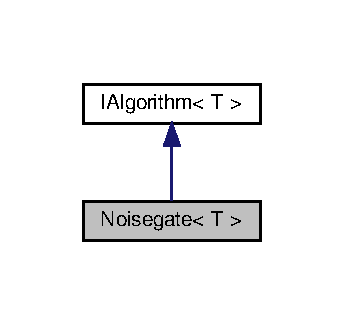
\includegraphics[width=165pt]{dc/d99/classNoisegate__inherit__graph}
\end{center}
\end{figure}


Collaboration diagram for Noisegate$<$ T $>$\+:
\nopagebreak
\begin{figure}[H]
\begin{center}
\leavevmode
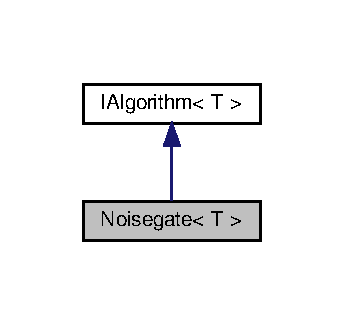
\includegraphics[width=165pt]{da/d40/classNoisegate__coll__graph}
\end{center}
\end{figure}
\subsection*{Public Member Functions}
\begin{DoxyCompactItemize}
\item 
\hyperlink{classNoisegate_a267d2fcf1167db41c925983401af2e6f}{Noisegate} (int threshold)
\item 
void \hyperlink{classNoisegate_a4ab84c99ea64beb3015134756a358eb9}{process\+Buffer} (T $\ast$buffer, int buffer\+Size) override
\end{DoxyCompactItemize}


\subsection{Detailed Description}
\subsubsection*{template$<$typename T$>$\newline
class Noisegate$<$ T $>$}

Authors\+: Parker True, Chris Fernandez, \& Ilana Macy Date Due\+: May 2, 2021 Assignment\+: Semester Project

applies echo effect to \hyperlink{classWav}{Wav} based on input delay 

\subsection{Constructor \& Destructor Documentation}
\mbox{\Hypertarget{classNoisegate_a267d2fcf1167db41c925983401af2e6f}\label{classNoisegate_a267d2fcf1167db41c925983401af2e6f}} 
\index{Noisegate@{Noisegate}!Noisegate@{Noisegate}}
\index{Noisegate@{Noisegate}!Noisegate@{Noisegate}}
\subsubsection{\texorpdfstring{Noisegate()}{Noisegate()}}
{\footnotesize\ttfamily template$<$typename T $>$ \\
\hyperlink{classNoisegate}{Noisegate}$<$ T $>$\+::\hyperlink{classNoisegate}{Noisegate} (\begin{DoxyParamCaption}\item[{int}]{threshold }\end{DoxyParamCaption})\hspace{0.3cm}{\ttfamily [inline]}, {\ttfamily [explicit]}}

constructs \hyperlink{classNoisegate}{Noisegate} processor 
\begin{DoxyParams}{Parameters}
{\em threshold} & threshold specified by user input \\
\hline
\end{DoxyParams}


\subsection{Member Function Documentation}
\mbox{\Hypertarget{classNoisegate_a4ab84c99ea64beb3015134756a358eb9}\label{classNoisegate_a4ab84c99ea64beb3015134756a358eb9}} 
\index{Noisegate@{Noisegate}!process\+Buffer@{process\+Buffer}}
\index{process\+Buffer@{process\+Buffer}!Noisegate@{Noisegate}}
\subsubsection{\texorpdfstring{process\+Buffer()}{processBuffer()}}
{\footnotesize\ttfamily template$<$typename T $>$ \\
void \hyperlink{classNoisegate}{Noisegate}$<$ T $>$\+::process\+Buffer (\begin{DoxyParamCaption}\item[{T $\ast$}]{buffer,  }\item[{int}]{buffer\+Size }\end{DoxyParamCaption})\hspace{0.3cm}{\ttfamily [inline]}, {\ttfamily [override]}, {\ttfamily [virtual]}}


\begin{DoxyParams}{Parameters}
{\em buffer} & pointer to audio buffer of type T \\
\hline
{\em buffer\+Size} & number of elements in audio buffer\\
\hline
\end{DoxyParams}
applies echo algorithm 

Implements \hyperlink{classIAlgorithm}{I\+Algorithm$<$ T $>$}.



The documentation for this class was generated from the following file\+:\begin{DoxyCompactItemize}
\item 
Noisegate.\+h\end{DoxyCompactItemize}

\hypertarget{classNormalization}{}\section{Normalization$<$ T $>$ Class Template Reference}
\label{classNormalization}\index{Normalization$<$ T $>$@{Normalization$<$ T $>$}}


{\ttfamily \#include $<$Normalization.\+h$>$}



Inheritance diagram for Normalization$<$ T $>$\+:
\nopagebreak
\begin{figure}[H]
\begin{center}
\leavevmode
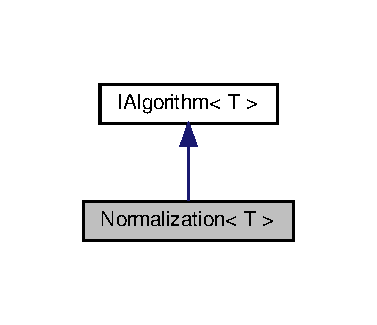
\includegraphics[width=181pt]{d2/d5e/classNormalization__inherit__graph}
\end{center}
\end{figure}


Collaboration diagram for Normalization$<$ T $>$\+:
\nopagebreak
\begin{figure}[H]
\begin{center}
\leavevmode
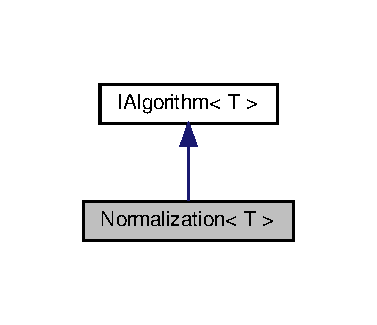
\includegraphics[width=181pt]{de/d74/classNormalization__coll__graph}
\end{center}
\end{figure}
\subsection*{Public Member Functions}
\begin{DoxyCompactItemize}
\item 
\hyperlink{classNormalization_a70f7d23e000cbdd8c0067a981b44ebe9}{Normalization} (int max)
\item 
int \hyperlink{classNormalization_a0ca4f15e6f0d23ec77c2946583e248b6}{find\+Max} (T $\ast$buffer, int buffer\+Size)
\item 
void \hyperlink{classNormalization_a0f441de817c3dbb8348cb9dfd66879d7}{process\+Buffer} (T $\ast$buffer, int buffer\+Size) override
\end{DoxyCompactItemize}


\subsection{Detailed Description}
\subsubsection*{template$<$typename T$>$\newline
class Normalization$<$ T $>$}

Authors\+: Parker True, Chris Fernandez, \& Ilana Macy Date Due\+: May 2, 2021 Assignment\+: Semester Project

applies normalization effect to \hyperlink{classWav}{Wav} based on input delay 

\subsection{Constructor \& Destructor Documentation}
\mbox{\Hypertarget{classNormalization_a70f7d23e000cbdd8c0067a981b44ebe9}\label{classNormalization_a70f7d23e000cbdd8c0067a981b44ebe9}} 
\index{Normalization@{Normalization}!Normalization@{Normalization}}
\index{Normalization@{Normalization}!Normalization@{Normalization}}
\subsubsection{\texorpdfstring{Normalization()}{Normalization()}}
{\footnotesize\ttfamily template$<$typename T $>$ \\
\hyperlink{classNormalization}{Normalization}$<$ T $>$\+::\hyperlink{classNormalization}{Normalization} (\begin{DoxyParamCaption}\item[{int}]{max }\end{DoxyParamCaption})\hspace{0.3cm}{\ttfamily [inline]}, {\ttfamily [explicit]}}

constructs \hyperlink{classNormalization}{Normalization} processor 
\begin{DoxyParams}{Parameters}
{\em new\+Max} & new maximum specified by user input \\
\hline
\end{DoxyParams}


\subsection{Member Function Documentation}
\mbox{\Hypertarget{classNormalization_a0ca4f15e6f0d23ec77c2946583e248b6}\label{classNormalization_a0ca4f15e6f0d23ec77c2946583e248b6}} 
\index{Normalization@{Normalization}!find\+Max@{find\+Max}}
\index{find\+Max@{find\+Max}!Normalization@{Normalization}}
\subsubsection{\texorpdfstring{find\+Max()}{findMax()}}
{\footnotesize\ttfamily template$<$typename T $>$ \\
int \hyperlink{classNormalization}{Normalization}$<$ T $>$\+::find\+Max (\begin{DoxyParamCaption}\item[{T $\ast$}]{buffer,  }\item[{int}]{buffer\+Size }\end{DoxyParamCaption})\hspace{0.3cm}{\ttfamily [inline]}}


\begin{DoxyParams}{Parameters}
{\em buffer} & pointer to audio buffer of type T \\
\hline
{\em buffer\+Size} & number of elements in audio buffer\\
\hline
\end{DoxyParams}
finds maximum value in buffer \mbox{\Hypertarget{classNormalization_a0f441de817c3dbb8348cb9dfd66879d7}\label{classNormalization_a0f441de817c3dbb8348cb9dfd66879d7}} 
\index{Normalization@{Normalization}!process\+Buffer@{process\+Buffer}}
\index{process\+Buffer@{process\+Buffer}!Normalization@{Normalization}}
\subsubsection{\texorpdfstring{process\+Buffer()}{processBuffer()}}
{\footnotesize\ttfamily template$<$typename T $>$ \\
void \hyperlink{classNormalization}{Normalization}$<$ T $>$\+::process\+Buffer (\begin{DoxyParamCaption}\item[{T $\ast$}]{buffer,  }\item[{int}]{buffer\+Size }\end{DoxyParamCaption})\hspace{0.3cm}{\ttfamily [inline]}, {\ttfamily [override]}, {\ttfamily [virtual]}}


\begin{DoxyParams}{Parameters}
{\em buffer} & pointer to audio buffer of type T \\
\hline
{\em buffer\+Size} & number of elements in audio buffer\\
\hline
\end{DoxyParams}
applies echo algorithm 

Implements \hyperlink{classIAlgorithm}{I\+Algorithm$<$ T $>$}.



The documentation for this class was generated from the following file\+:\begin{DoxyCompactItemize}
\item 
Normalization.\+h\end{DoxyCompactItemize}

\hypertarget{classWav}{}\section{Wav Class Reference}
\label{classWav}\index{Wav@{Wav}}


{\ttfamily \#include $<$Wav.\+h$>$}

\subsection*{Public Member Functions}
\begin{DoxyCompactItemize}
\item 
\hyperlink{classWav_a573605770be554fbf416e72e0f9109fe}{Wav} (const std\+::string \&, const std\+::string \&)
\item 
virtual \hyperlink{classWav_a1510b246ba121b103a60b8e7839af25f}{$\sim$\+Wav} ()
\item 
\mbox{\Hypertarget{classWav_a038085c64b750429419523e58cef4a90}\label{classWav_a038085c64b750429419523e58cef4a90}} 
void {\bfseries destruct\+Data} ()
\item 
void \hyperlink{classWav_a6569b629ca9e46d0093f8bfd23d92735}{write\+File} (std\+::vector$<$ std\+::string $>$ \&)
\item 
void \hyperlink{classWav_a6f8162ea823152663dd7f556612c220e}{write\+C\+SV} (std\+::vector$<$ \hyperlink{classWav}{Wav} $\ast$$>$)
\item 
void \hyperlink{classWav_a52240b5a0803b1fd074b98d79b51e589}{print\+Metadata} ()
\item 
std\+::string \hyperlink{classWav_ab091dcb5c70b025779d4073e344e60f2}{get\+File\+Name} () const
\item 
int \hyperlink{classWav_af3aaf1636defa1288d866725e39c7f69}{get\+Bits\+Per\+Sample} () const
\item 
int \hyperlink{classWav_a71fdfa1d9f5e7c1b86f07bbff4249dca}{get\+Buffer\+Size} () const
\item 
{\footnotesize template$<$typename T $>$ }\\T $\ast$ \hyperlink{classWav_ac236b8cc7453f5dd6cc0623b5c200bee}{get\+Buffer} () const
\item 
{\footnotesize template$<$typename T $>$ }\\T $\ast$ \hyperlink{classWav_aca22bfd496dad7ecf80e17a691ab1c4c}{get\+Buffer2} () const
\end{DoxyCompactItemize}


\subsection{Detailed Description}
Authors\+: Parker True, Chris Fernandez, \& Ilana Macy Date Due\+: May 2, 2021 Assignment\+: Semester Project 

\subsection{Constructor \& Destructor Documentation}
\mbox{\Hypertarget{classWav_a573605770be554fbf416e72e0f9109fe}\label{classWav_a573605770be554fbf416e72e0f9109fe}} 
\index{Wav@{Wav}!Wav@{Wav}}
\index{Wav@{Wav}!Wav@{Wav}}
\subsubsection{\texorpdfstring{Wav()}{Wav()}}
{\footnotesize\ttfamily Wav\+::\+Wav (\begin{DoxyParamCaption}\item[{const std\+::string \&}]{path,  }\item[{const std\+::string \&}]{file\+Name }\end{DoxyParamCaption})}


\begin{DoxyParams}{Parameters}
{\em file\+Name} & -\/ the name of the file constructs \hyperlink{classWav}{Wav} object from input file \\
\hline
\end{DoxyParams}
\mbox{\Hypertarget{classWav_a1510b246ba121b103a60b8e7839af25f}\label{classWav_a1510b246ba121b103a60b8e7839af25f}} 
\index{Wav@{Wav}!````~Wav@{$\sim$\+Wav}}
\index{````~Wav@{$\sim$\+Wav}!Wav@{Wav}}
\subsubsection{\texorpdfstring{$\sim$\+Wav()}{~Wav()}}
{\footnotesize\ttfamily Wav\+::$\sim$\+Wav (\begin{DoxyParamCaption}{ }\end{DoxyParamCaption})\hspace{0.3cm}{\ttfamily [virtual]}}


\begin{DoxyItemize}
\item destruct \hyperlink{classWav}{Wav} object and delete buffer 
\end{DoxyItemize}

\subsection{Member Function Documentation}
\mbox{\Hypertarget{classWav_af3aaf1636defa1288d866725e39c7f69}\label{classWav_af3aaf1636defa1288d866725e39c7f69}} 
\index{Wav@{Wav}!get\+Bits\+Per\+Sample@{get\+Bits\+Per\+Sample}}
\index{get\+Bits\+Per\+Sample@{get\+Bits\+Per\+Sample}!Wav@{Wav}}
\subsubsection{\texorpdfstring{get\+Bits\+Per\+Sample()}{getBitsPerSample()}}
{\footnotesize\ttfamily int Wav\+::get\+Bits\+Per\+Sample (\begin{DoxyParamCaption}{ }\end{DoxyParamCaption}) const}

\begin{DoxyReturn}{Returns}
-\/ number of bits per sample 
\end{DoxyReturn}
\mbox{\Hypertarget{classWav_ac236b8cc7453f5dd6cc0623b5c200bee}\label{classWav_ac236b8cc7453f5dd6cc0623b5c200bee}} 
\index{Wav@{Wav}!get\+Buffer@{get\+Buffer}}
\index{get\+Buffer@{get\+Buffer}!Wav@{Wav}}
\subsubsection{\texorpdfstring{get\+Buffer()}{getBuffer()}}
{\footnotesize\ttfamily template$<$typename T $>$ \\
T$\ast$ Wav\+::get\+Buffer (\begin{DoxyParamCaption}{ }\end{DoxyParamCaption}) const\hspace{0.3cm}{\ttfamily [inline]}}

\begin{DoxyReturn}{Returns}
-\/ pointer to buffer of type T 
\end{DoxyReturn}
\mbox{\Hypertarget{classWav_aca22bfd496dad7ecf80e17a691ab1c4c}\label{classWav_aca22bfd496dad7ecf80e17a691ab1c4c}} 
\index{Wav@{Wav}!get\+Buffer2@{get\+Buffer2}}
\index{get\+Buffer2@{get\+Buffer2}!Wav@{Wav}}
\subsubsection{\texorpdfstring{get\+Buffer2()}{getBuffer2()}}
{\footnotesize\ttfamily template$<$typename T $>$ \\
T$\ast$ Wav\+::get\+Buffer2 (\begin{DoxyParamCaption}{ }\end{DoxyParamCaption}) const\hspace{0.3cm}{\ttfamily [inline]}}

\begin{DoxyReturn}{Returns}
-\/ pointer to buffer2 of type T 
\end{DoxyReturn}
\mbox{\Hypertarget{classWav_a71fdfa1d9f5e7c1b86f07bbff4249dca}\label{classWav_a71fdfa1d9f5e7c1b86f07bbff4249dca}} 
\index{Wav@{Wav}!get\+Buffer\+Size@{get\+Buffer\+Size}}
\index{get\+Buffer\+Size@{get\+Buffer\+Size}!Wav@{Wav}}
\subsubsection{\texorpdfstring{get\+Buffer\+Size()}{getBufferSize()}}
{\footnotesize\ttfamily int Wav\+::get\+Buffer\+Size (\begin{DoxyParamCaption}{ }\end{DoxyParamCaption}) const}

\begin{DoxyReturn}{Returns}
-\/ size of (each) unsigned char buffer 
\end{DoxyReturn}
\mbox{\Hypertarget{classWav_ab091dcb5c70b025779d4073e344e60f2}\label{classWav_ab091dcb5c70b025779d4073e344e60f2}} 
\index{Wav@{Wav}!get\+File\+Name@{get\+File\+Name}}
\index{get\+File\+Name@{get\+File\+Name}!Wav@{Wav}}
\subsubsection{\texorpdfstring{get\+File\+Name()}{getFileName()}}
{\footnotesize\ttfamily std\+::string Wav\+::get\+File\+Name (\begin{DoxyParamCaption}{ }\end{DoxyParamCaption}) const}

\begin{DoxyReturn}{Returns}
-\/ name of .wav file 
\end{DoxyReturn}
\mbox{\Hypertarget{classWav_a52240b5a0803b1fd074b98d79b51e589}\label{classWav_a52240b5a0803b1fd074b98d79b51e589}} 
\index{Wav@{Wav}!print\+Metadata@{print\+Metadata}}
\index{print\+Metadata@{print\+Metadata}!Wav@{Wav}}
\subsubsection{\texorpdfstring{print\+Metadata()}{printMetadata()}}
{\footnotesize\ttfamily void Wav\+::print\+Metadata (\begin{DoxyParamCaption}{ }\end{DoxyParamCaption})}

prints each metadata on newline \mbox{\Hypertarget{classWav_a6f8162ea823152663dd7f556612c220e}\label{classWav_a6f8162ea823152663dd7f556612c220e}} 
\index{Wav@{Wav}!write\+C\+SV@{write\+C\+SV}}
\index{write\+C\+SV@{write\+C\+SV}!Wav@{Wav}}
\subsubsection{\texorpdfstring{write\+C\+S\+V()}{writeCSV()}}
{\footnotesize\ttfamily void Wav\+::write\+C\+SV (\begin{DoxyParamCaption}\item[{std\+::vector$<$ \hyperlink{classWav}{Wav} $\ast$$>$}]{wavs }\end{DoxyParamCaption})}

writes to output csv file \mbox{\Hypertarget{classWav_a6569b629ca9e46d0093f8bfd23d92735}\label{classWav_a6569b629ca9e46d0093f8bfd23d92735}} 
\index{Wav@{Wav}!write\+File@{write\+File}}
\index{write\+File@{write\+File}!Wav@{Wav}}
\subsubsection{\texorpdfstring{write\+File()}{writeFile()}}
{\footnotesize\ttfamily void Wav\+::write\+File (\begin{DoxyParamCaption}\item[{std\+::vector$<$ std\+::string $>$ \&}]{file\+Names }\end{DoxyParamCaption})}


\begin{DoxyParams}{Parameters}
{\em file\+Names} & -\/ vector containing list of filenames already in directory writes contents of \hyperlink{classWav}{Wav} object to output .wav file \\
\hline
\end{DoxyParams}


The documentation for this class was generated from the following files\+:\begin{DoxyCompactItemize}
\item 
Wav.\+h\item 
Wav.\+cpp\end{DoxyCompactItemize}

\hypertarget{structWavHeader}{}\section{Wav\+Header Struct Reference}
\label{structWavHeader}\index{Wav\+Header@{Wav\+Header}}


{\ttfamily \#include $<$Wav\+Header.\+h$>$}

\subsection*{Public Attributes}
\begin{DoxyCompactItemize}
\item 
\mbox{\Hypertarget{structWavHeader_ae0965a20455681050284337f890e1345}\label{structWavHeader_ae0965a20455681050284337f890e1345}} 
char {\bfseries riff\+ID} \mbox{[}4\mbox{]}
\item 
\mbox{\Hypertarget{structWavHeader_a303a922a318e59a008486d200278642e}\label{structWavHeader_a303a922a318e59a008486d200278642e}} 
int {\bfseries file\+Size}
\item 
\mbox{\Hypertarget{structWavHeader_a87ded76921fcfbb0b79530a2d907e1a6}\label{structWavHeader_a87ded76921fcfbb0b79530a2d907e1a6}} 
char {\bfseries wave\+ID} \mbox{[}4\mbox{]}
\item 
\mbox{\Hypertarget{structWavHeader_afd86c492cd7479eb92ad528757a31c1a}\label{structWavHeader_afd86c492cd7479eb92ad528757a31c1a}} 
char {\bfseries fmt\+ID} \mbox{[}4\mbox{]}
\item 
\mbox{\Hypertarget{structWavHeader_a01300c585ceede02c336d7cc32eb9b43}\label{structWavHeader_a01300c585ceede02c336d7cc32eb9b43}} 
int {\bfseries fmt\+Size}
\item 
\mbox{\Hypertarget{structWavHeader_ada5498f780f96cb417d2e62b4cd42c30}\label{structWavHeader_ada5498f780f96cb417d2e62b4cd42c30}} 
short {\bfseries audio\+Fmt}
\item 
\mbox{\Hypertarget{structWavHeader_a974f24ee8f6c0f7a6a881b1b5f917bfa}\label{structWavHeader_a974f24ee8f6c0f7a6a881b1b5f917bfa}} 
short {\bfseries num\+Channels}
\item 
\mbox{\Hypertarget{structWavHeader_a70f6545b7646e8f9c2f02118150566d1}\label{structWavHeader_a70f6545b7646e8f9c2f02118150566d1}} 
int {\bfseries sample\+Rate}
\item 
\mbox{\Hypertarget{structWavHeader_ab9c193dd57da1a877cd5193657ed8a75}\label{structWavHeader_ab9c193dd57da1a877cd5193657ed8a75}} 
int {\bfseries byte\+Rate}
\item 
\mbox{\Hypertarget{structWavHeader_a1bfbf825695b7626f58e64355a3ee4b1}\label{structWavHeader_a1bfbf825695b7626f58e64355a3ee4b1}} 
short {\bfseries block\+Align}
\item 
\mbox{\Hypertarget{structWavHeader_a2dbf27f9cd07e02e744d4f71bc25109b}\label{structWavHeader_a2dbf27f9cd07e02e744d4f71bc25109b}} 
short {\bfseries bits\+Per\+Sample}
\item 
\mbox{\Hypertarget{structWavHeader_ad0ff2115c45221d8a763356de04de028}\label{structWavHeader_ad0ff2115c45221d8a763356de04de028}} 
char {\bfseries data\+ID} \mbox{[}4\mbox{]}
\item 
\mbox{\Hypertarget{structWavHeader_a501041ecccd8debd17d35e5d59844164}\label{structWavHeader_a501041ecccd8debd17d35e5d59844164}} 
int {\bfseries data\+Size}
\end{DoxyCompactItemize}


\subsection{Detailed Description}
Authors\+: Parker True, Chris Fernandez, \& Ilana Macy Date Due\+: May 2, 2021 Assignment\+: Semester Project 

The documentation for this struct was generated from the following file\+:\begin{DoxyCompactItemize}
\item 
Wav\+Header.\+h\end{DoxyCompactItemize}

\hypertarget{classWavManager}{}\section{Wav\+Manager Class Reference}
\label{classWavManager}\index{Wav\+Manager@{Wav\+Manager}}


{\ttfamily \#include $<$Wav\+Manager.\+h$>$}

\subsection*{Public Member Functions}
\begin{DoxyCompactItemize}
\item 
\hyperlink{classWavManager_ae9e3c60a5f1744cf93d8c5a7e81ec279}{Wav\+Manager} (char $\ast$)
\item 
virtual \hyperlink{classWavManager_ada2c41fa0b1f388b3d90ade85fd21f6a}{$\sim$\+Wav\+Manager} ()
\item 
\hyperlink{classWav}{Wav} $\ast$ \hyperlink{classWavManager_a81286b348dd7d7969cfffebc0197e457}{get\+Wav} (int) const
\item 
int \hyperlink{classWavManager_a92aeb164533efeefd7d636b3da5b2828}{get\+Size} () const
\item 
\hyperlink{classWav}{Wav} $\ast$ \hyperlink{classWavManager_a30d87e1568d7fcdcf81089c8125819d1}{select\+Wav} ()
\item 
std\+::vector$<$ \hyperlink{classWav}{Wav} $\ast$ $>$ \hyperlink{classWavManager_af4ca861d89e3aceab92629958223784a}{get\+Wavs} () const
\item 
std\+::vector$<$ std\+::string $>$ \hyperlink{classWavManager_a505c8ecc7ae96bc5c6faad602ac26a6c}{get\+File\+Names} () const
\end{DoxyCompactItemize}


\subsection{Detailed Description}
Authors\+: Parker True, Chris Fernandez, \& Ilana Macy Date Due\+: May 2, 2021 Assignment\+: Semester Project


\begin{DoxyItemize}
\item manages input, storage, and output for \hyperlink{classWav}{Wav} files 
\end{DoxyItemize}

\subsection{Constructor \& Destructor Documentation}
\mbox{\Hypertarget{classWavManager_ae9e3c60a5f1744cf93d8c5a7e81ec279}\label{classWavManager_ae9e3c60a5f1744cf93d8c5a7e81ec279}} 
\index{Wav\+Manager@{Wav\+Manager}!Wav\+Manager@{Wav\+Manager}}
\index{Wav\+Manager@{Wav\+Manager}!Wav\+Manager@{Wav\+Manager}}
\subsubsection{\texorpdfstring{Wav\+Manager()}{WavManager()}}
{\footnotesize\ttfamily Wav\+Manager\+::\+Wav\+Manager (\begin{DoxyParamCaption}\item[{char $\ast$}]{path }\end{DoxyParamCaption})}


\begin{DoxyParams}{Parameters}
{\em path} & -\/ the directory path it should take\\
\hline
\end{DoxyParams}

\begin{DoxyItemize}
\item construct \hyperlink{classWavManager}{Wav\+Manager} object given path to directory of .wav files 
\end{DoxyItemize}\mbox{\Hypertarget{classWavManager_ada2c41fa0b1f388b3d90ade85fd21f6a}\label{classWavManager_ada2c41fa0b1f388b3d90ade85fd21f6a}} 
\index{Wav\+Manager@{Wav\+Manager}!````~Wav\+Manager@{$\sim$\+Wav\+Manager}}
\index{````~Wav\+Manager@{$\sim$\+Wav\+Manager}!Wav\+Manager@{Wav\+Manager}}
\subsubsection{\texorpdfstring{$\sim$\+Wav\+Manager()}{~WavManager()}}
{\footnotesize\ttfamily Wav\+Manager\+::$\sim$\+Wav\+Manager (\begin{DoxyParamCaption}{ }\end{DoxyParamCaption})\hspace{0.3cm}{\ttfamily [virtual]}}


\begin{DoxyItemize}
\item destructs \hyperlink{classWavManager}{Wav\+Manager} and deletes all \hyperlink{classWav}{Wav} files in wavs vector 
\end{DoxyItemize}

\subsection{Member Function Documentation}
\mbox{\Hypertarget{classWavManager_a505c8ecc7ae96bc5c6faad602ac26a6c}\label{classWavManager_a505c8ecc7ae96bc5c6faad602ac26a6c}} 
\index{Wav\+Manager@{Wav\+Manager}!get\+File\+Names@{get\+File\+Names}}
\index{get\+File\+Names@{get\+File\+Names}!Wav\+Manager@{Wav\+Manager}}
\subsubsection{\texorpdfstring{get\+File\+Names()}{getFileNames()}}
{\footnotesize\ttfamily std\+::vector$<$ std\+::string $>$ Wav\+Manager\+::get\+File\+Names (\begin{DoxyParamCaption}{ }\end{DoxyParamCaption}) const}

\begin{DoxyReturn}{Returns}
file\+Names vector 
\end{DoxyReturn}
\mbox{\Hypertarget{classWavManager_a92aeb164533efeefd7d636b3da5b2828}\label{classWavManager_a92aeb164533efeefd7d636b3da5b2828}} 
\index{Wav\+Manager@{Wav\+Manager}!get\+Size@{get\+Size}}
\index{get\+Size@{get\+Size}!Wav\+Manager@{Wav\+Manager}}
\subsubsection{\texorpdfstring{get\+Size()}{getSize()}}
{\footnotesize\ttfamily int Wav\+Manager\+::get\+Size (\begin{DoxyParamCaption}{ }\end{DoxyParamCaption}) const}

\begin{DoxyReturn}{Returns}
-\/ size of wavs vector 
\end{DoxyReturn}
\mbox{\Hypertarget{classWavManager_a81286b348dd7d7969cfffebc0197e457}\label{classWavManager_a81286b348dd7d7969cfffebc0197e457}} 
\index{Wav\+Manager@{Wav\+Manager}!get\+Wav@{get\+Wav}}
\index{get\+Wav@{get\+Wav}!Wav\+Manager@{Wav\+Manager}}
\subsubsection{\texorpdfstring{get\+Wav()}{getWav()}}
{\footnotesize\ttfamily \hyperlink{classWav}{Wav} $\ast$ Wav\+Manager\+::get\+Wav (\begin{DoxyParamCaption}\item[{int}]{i }\end{DoxyParamCaption}) const}


\begin{DoxyParams}{Parameters}
{\em i} & -\/ index i \\
\hline
\end{DoxyParams}
\begin{DoxyReturn}{Returns}
-\/ pointer to \hyperlink{classWav}{Wav} object at index i in wavs vector 
\end{DoxyReturn}
\mbox{\Hypertarget{classWavManager_af4ca861d89e3aceab92629958223784a}\label{classWavManager_af4ca861d89e3aceab92629958223784a}} 
\index{Wav\+Manager@{Wav\+Manager}!get\+Wavs@{get\+Wavs}}
\index{get\+Wavs@{get\+Wavs}!Wav\+Manager@{Wav\+Manager}}
\subsubsection{\texorpdfstring{get\+Wavs()}{getWavs()}}
{\footnotesize\ttfamily std\+::vector$<$ \hyperlink{classWav}{Wav} $\ast$ $>$ Wav\+Manager\+::get\+Wavs (\begin{DoxyParamCaption}{ }\end{DoxyParamCaption}) const}

\begin{DoxyReturn}{Returns}
wavs vector 
\end{DoxyReturn}
\mbox{\Hypertarget{classWavManager_a30d87e1568d7fcdcf81089c8125819d1}\label{classWavManager_a30d87e1568d7fcdcf81089c8125819d1}} 
\index{Wav\+Manager@{Wav\+Manager}!select\+Wav@{select\+Wav}}
\index{select\+Wav@{select\+Wav}!Wav\+Manager@{Wav\+Manager}}
\subsubsection{\texorpdfstring{select\+Wav()}{selectWav()}}
{\footnotesize\ttfamily \hyperlink{classWav}{Wav} $\ast$ Wav\+Manager\+::select\+Wav (\begin{DoxyParamCaption}{ }\end{DoxyParamCaption})}

\begin{DoxyReturn}{Returns}
-\/ pointer to the \hyperlink{classWav}{Wav} object you select 
\end{DoxyReturn}


The documentation for this class was generated from the following files\+:\begin{DoxyCompactItemize}
\item 
Wav\+Manager.\+h\item 
Wav\+Manager.\+cpp\end{DoxyCompactItemize}

\chapter{File Documentation}
\hypertarget{main_8cpp}{}\section{main.\+cpp File Reference}
\label{main_8cpp}\index{main.\+cpp@{main.\+cpp}}
{\ttfamily \#include \char`\"{}Wav\+Manager.\+h\char`\"{}}\newline
{\ttfamily \#include \char`\"{}Driver.\+h\char`\"{}}\newline
Include dependency graph for main.\+cpp\+:
\nopagebreak
\begin{figure}[H]
\begin{center}
\leavevmode
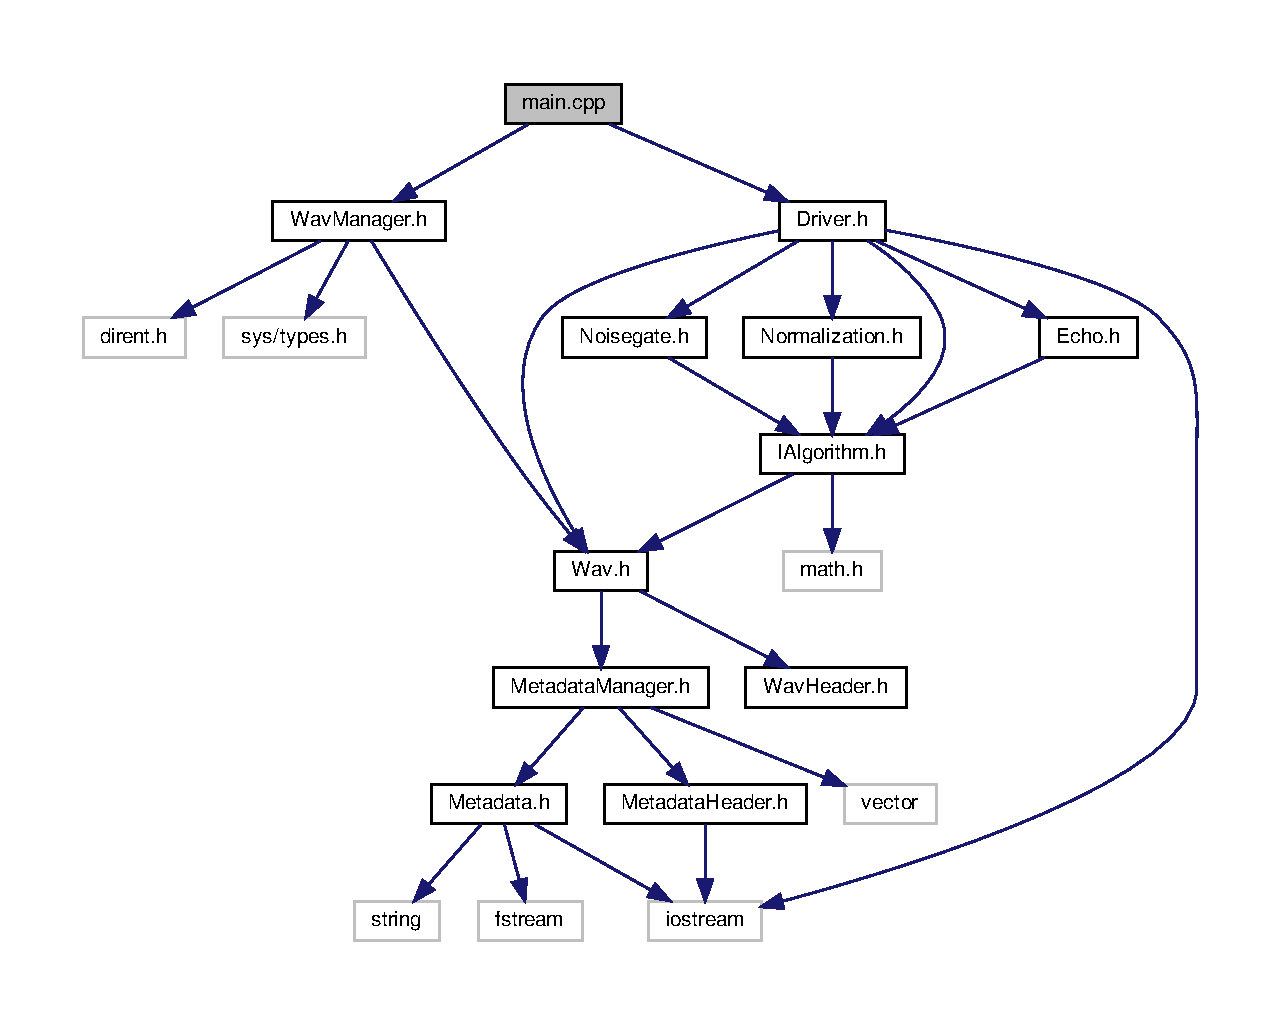
\includegraphics[width=350pt]{da/dce/main_8cpp__incl}
\end{center}
\end{figure}
\subsection*{Functions}
\begin{DoxyCompactItemize}
\item 
void \hyperlink{main_8cpp_ad9d0e397081801b3c81f84aef014b9ca}{fn} ()
\begin{DoxyCompactList}\small\item\em The function bar. \end{DoxyCompactList}\item 
int \hyperlink{main_8cpp_af3ed9c200de85b53c94cd18764b246a2}{main} (int argc, char $\ast$const argv\mbox{[}$\,$\mbox{]})
\end{DoxyCompactItemize}


\subsection{Detailed Description}
Authors\+: Parker True, Chris Fernandez, \& Ilana Macy Date Due\+: May 2, 2021 Assignment\+: Semester Project 

\subsection{Function Documentation}
\mbox{\Hypertarget{main_8cpp_ad9d0e397081801b3c81f84aef014b9ca}\label{main_8cpp_ad9d0e397081801b3c81f84aef014b9ca}} 
\index{main.\+cpp@{main.\+cpp}!fn@{fn}}
\index{fn@{fn}!main.\+cpp@{main.\+cpp}}
\subsubsection{\texorpdfstring{fn()}{fn()}}
{\footnotesize\ttfamily void fn (\begin{DoxyParamCaption}{ }\end{DoxyParamCaption})}



The function bar. 

This function does something which is doing nothing. So this text is totally senseless and you really do not need to read this, because this text is basically saying nothing.

\begin{DoxyNote}{Note}
This text shall only show you, how such a "note" section is looking. There is nothing which really needs your notice, so you do not really need to read this section.
\end{DoxyNote}

\begin{DoxyParams}[1]{Parameters}
\mbox{\tt in}  & {\em a} & Description of parameter a. \\
\hline
\mbox{\tt out}  & {\em b} & Description of the parameter b. \\
\hline
\mbox{\tt in,out}  & {\em c} & Description of the parameter c.\\
\hline
\end{DoxyParams}
\begin{DoxyReturn}{Returns}
The error return code of the function.
\end{DoxyReturn}

\begin{DoxyRetVals}{Return values}
{\em E\+R\+R\+\_\+\+S\+U\+C\+C\+E\+SS} & The function is successfully executed \\
\hline
{\em E\+R\+R\+\_\+\+F\+A\+I\+L\+U\+RE} & An error occurred Purpose of function What does it do \\
\hline
\end{DoxyRetVals}
\mbox{\Hypertarget{main_8cpp_af3ed9c200de85b53c94cd18764b246a2}\label{main_8cpp_af3ed9c200de85b53c94cd18764b246a2}} 
\index{main.\+cpp@{main.\+cpp}!main@{main}}
\index{main@{main}!main.\+cpp@{main.\+cpp}}
\subsubsection{\texorpdfstring{main()}{main()}}
{\footnotesize\ttfamily int main (\begin{DoxyParamCaption}\item[{int}]{argc,  }\item[{char $\ast$const}]{argv\mbox{[}$\,$\mbox{]} }\end{DoxyParamCaption})}


\begin{DoxyParams}{Parameters}
{\em argc} & number of command line arguments \\
\hline
{\em argv} & array of command line arguments \\
\hline
\end{DoxyParams}
\begin{DoxyReturn}{Returns}
0 
\end{DoxyReturn}

%--- End generated contents ---

% Index
\backmatter
\newpage
\phantomsection
\clearemptydoublepage
\addcontentsline{toc}{chapter}{Index}
\printindex

\end{document}
